\section{Architecture}
\label{sec_arch}

In this section we discuss the over all architecture of the proposed FPGA based neural network prototyping platform and the specific implementation of the approximate probabilistic neural network~(FAPNN) library.

\subsection{System Architecture}

\begin{figure}[t]
\centering
   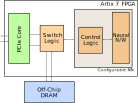
\includegraphics[height=0.7\columnwidth]{Figures/systemarch.pdf}
   \caption{Architecture of the proposed FPGA based neural network evaluation platform}
   \label{fig:sysArch}
\end{figure}

The system-level architecture of the proposed FPGA-based neural network accelerator platform is as shown in Fig.~\ref{fig:sysArch}.
It is implemented on an off-the-shelf vendor supported FPGA development board (Xilinx~AC701).
The FPGA communicates with a standard host computer through PCIexpress interface to send data samples and to receive the processed output.
For the chosen platform, this communication link provides up to 2 GB/s communication bandwidth.
The FPGA board also has an on-board DDR3 memory supporting up to 1GB for temporary data storage.

We use our previously developed open-source FPGA switch IP core for interfacing the PCIe core, DRAM memory controller and the neural network accelerator~\cite{blanked}.
Through software control from the host, the training data, weights and test data can be either stored in the DRAM or directly injected to the neural network.
For the PNN implementation, the data is directly injected to the neural network since the modified architecture is capable of storing the entire training data in the FPGA itself.
The interfacing logic (PCIe and DRAM) and the switch logic remains the same irrespective of the neural network implemented on the FPGA platform.

The control logic block shown in Fig.~\ref{fig:sysArch} is specific to the target neural network architecture.
It is responsible for generating the global control signals, which controls the storage of weights (training data in case of PNN) inside the appropriate neurons.
It also acts as the input later for PNN where it accepts data from the switch and converts it into the specific format required by the neural network.
In the present implementation, the host computer sends normalised data for both training and testing purposes.

The neural network block implements all the remaining layers of the neural network, such as pattern, summation and output layers of the PNN.
The number of classes in the pattern layer and the number of neurons in each class can be configured at design time.
The automation tool automatically generates the HDL code corresponding to the chosen parameters.

\subsection{FAPNN}
FAPNN is available in the form of a library targeting the proposed system architecture.
Its components are highly customisable and scalable at design time based on user requirements.
Following similar design principles, library components can be developed for implementing other neural network models.
Irrespective of the model, the interface between the neural network and the remainder of the system remains unaltered.
In the subsequent section we detail the individual building blocks of FAPNN.

\subsubsection{\bf Neuron}
\begin{figure}[t]
\centering
   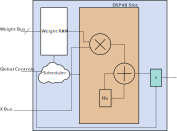
\includegraphics[height=0.6\columnwidth]{Figures/neuron.pdf}
   \caption{Architecture of a single Neuron using Xilinx DSP48 slice}
   \label{fig:neuron}
\end{figure}
The architecture of a single neuron used in the PNN pattern layer is depicted in Fig.~\ref{fig:neuron}.
Internally each neuron instantiates a Xilinx DSP48E1 slice.
DSP48E1 is a built-in hard macro available in Xilinx 7-Series FPGAs, which are highly efficient in implementing signal processing tasks.
It has a 25$\times$25 multiplier and a 48-bit accumulator.
In the proposed architecture, each neuron implements a single DSP slice irrespective of the size of the feature vecor (X).
The same slice is used multiple times under the control of a scheduler logic to multiply with different weights ($w_{i}$) with corresponding feature ($x_{i}$).
The internal accumulator of the DSP slice accumulates the result of multiplication, emulating the dot product.
This makes the design highly scalable enabling concurrent implementation large number of neurons in the pattern layer, supporting large number of training samples.
The drawback is this resource sharing incurs a clock latency equal to the number of features for each input sample.
This is mitigated by the high clock frequency at which the overall system is operating.

The neuron internally implements a memory block called \emph{Weight RAM} for storing the multiplication weights (training data).
Each location in the memory is 16-bit wide and the depth of the memory can be configured at design time as the size of the feature vector.
During training, the weights are stored in the appropriate memory location by the scheduler.
It uses the control signals from the Control logic to decide whether the input data should be considered as training data to store in the memory or as test data.
During testing, the scheduler sequentially reads data from the Weight RAM and applies it to the DSP slice input for multiplying with the input data.

The input data bus width to the neuron is 16-bits and in the PNN implementation data is represented using fixed point notation.
Although the accuracy may be affected by fixed point representation compared to floating point representation, the hardware cost is much reduced and the clock frequency is improved.

Finally the comparator ($f$ block in the figure) decides the output of the neuron based on the activation function.
Traditional PNNs employ an exponential function to generate the output from the pattern layer as discussed in Section~\ref{sec_related}.
As discussed before, implementation of exponential functions are high resource intensive which limits the number of neurons in the pattern layer.
Researchers have previously implemented it using look-up-tables~(LUTs) or special IP cores such as CORDIC~(coordinate rotational digital computer).
For simplification, we use a threshold based activation function.
Mathematically it can be represented as


\begin{figure}[t]
\centering
   \includegraphics[height=0.45\columnwidth]{Figures/pdf.pdf}
   \caption{Approximation of probability density function}
   \label{fig:pdf}
\end{figure}

\begin{equation}
\label{e2}
 g_{i}=
  \begin{cases}
    1       & \quad \text{if } \quad {\boldsymbol{X\cdot W_{i}}} > \theta \\
    0  & \quad \text{otherwise} 
  \end{cases}
\end{equation}
where $\theta$ is a threshold value.
This approximation greatly reduces the hardware complexity at the same time is supported by the previous research.
In the original work were PNN was introduced~\citep{specht1990}, the validity of this function is acknowledged.
The exact form of the activation function is not critical to the usefulness of the network. 
Since the data is normalised, the value of the dot product is always between 0 and 1.
The common criteria is that the activation function takes its maximum value at $X.W_i$ = 1 or maximum similarity between the input pattern X and the pattern stored in the pattern unit; the activation function decreases as the pattern becomes less similar.
Mathematically for a two feature input data, the probability density function changes its shape from Gaussian to square prism when the activation function is approximated as shown in Fig.~\ref{fig:pdf}.
The value of $\theta$ is decided during training through cross validation sub-training data.

\subsubsection{\bf Averaging Neuron}
For every class, an averaging neuron is instantiated for summing up and finding the average of the pattern neurons.
Since the approximation makes the output of the pattern neuron to be either 1 or 0, the averaging neuron has to implement only one bit adders.
This greatly reduces the resource requirement.
In the present implementation adders are not resource shared and all of them are concurrently implemented.
The output of the this neuron is a 16-bit fixed point representation of the average probability of all the pattern neurons for a specific class.

\subsubsection{\bf Output Neuron}
The output neuron implements a simple comparator to decide the highest value among all the averaging neurons.
The number of inputs to this neuron depends upon the number of classes.
The output of this neuron is the binary number representation of the class with the highest probability.

\subsection{Design Automation} 

\begin{figure}[t]
\centering
   \includegraphics[height=0.6\columnwidth]{Figures/toolFlow.pdf}
   \caption{Tool flow for the proposed FAPNN platform}
   \label{fig:toolFlow}
\end{figure}

The proposed platform provides design automation support for quickly prototyping the FAPNN on real hardware.
The designer provides two design parameters such as the number of classes and the number of neurons in each class through a Python based automation tool.
Based on these parameters, the automation script generates the Verilog HDL code corresponding to FAPNN.
It then automatically interfaces FAPNN with the code base corresponding to the communication infrastructure.
It then uses the FPGA vendor (Xilinx) specific tool flow for implementing the design for a target FPGA platform.
The overall tool-flow is shown in Fig.~\ref{fig:toolFlow}